%------------------------------------------
% Isometric Logratio Transform
%
%------------------------------------------
% About:
% Notes for the Isometric Logratio
% Transformation and its application to
% compositional data analysis.
%
%------------------------------------------
% Author:
% R. Nate Crummett
%------------------------------------------
\documentclass[dark]{cgem-presentation}

% Link to figures directory
\graphicspath{{./Figs}{./Logo}}

\addbibresource{Bib/egozcue2003.bib}
\addbibresource{Bib/pearson1897.bib}
\addbibresource{Bib/pawlowsky-glahn2007.bib}
\addbibresource{Bib/aitchison2005.bib}
\addbibresource{Bib/chave2017.bib}

\DeclareMathOperator{\closure}{\operatorname{\mathcal{C}}}
\DeclareMathOperator{\alr}{\operatorname{alr}}
\DeclareMathOperator{\clr}{\operatorname{clr}}
\DeclareMathOperator{\ilr}{\operatorname{ilr}}
\DeclareMathOperator{\range}{\operatorname{range}}
\DeclareMathOperator{\mnull}{\operatorname{null}}

%------------------------------------------
%% Presentation
\begin{document}

% Title slide
\begin{frame}[plain]
	% Title frame text
	\begin{center}
		% Title 
		\vspace{1cm}
		\Huge
		Compositional Data Analysis Notes

		\vspace{1cm}
		% Authors
		\textcolor{SecondColor}{\huge R Nate Crummett }

		\vspace{2.5cm}
		% Affiliations
		{ \color{SecondColor}
		\itshape
		\Large
		Center for Gravity, Electric \& Magnetic Studies (CGEM)

		\vspace{-5mm}
		\large
		Department of Geophysics --- Colorado School of Mines
		}

		\vspace{2mm}
		\large
		\today
	\end{center}

	% Title page Mines logo
	\begin{figure}
		\begin{textblock*}{2.7cm}(0.06\paperwidth,0.34\paperheight)
			\includegraphics[width=2.7cm]{\LogoFileMines}
		\end{textblock*}
	\end{figure}

	% Title page CGEM logo
	\begin{figure}
		\vspace*{-11.09294pt}
		\begin{textblock*}{2.85cm}(0.77\paperwidth,0.36\paperheight)
			\includegraphics[width=2.4cm,keepaspectratio]{\LogoFileCGEM}
		\end{textblock*}
	\end{figure}
\end{frame}

\begin{frame}[plain]
	\large
	\vspace{6mm}
	\begin{figure}
		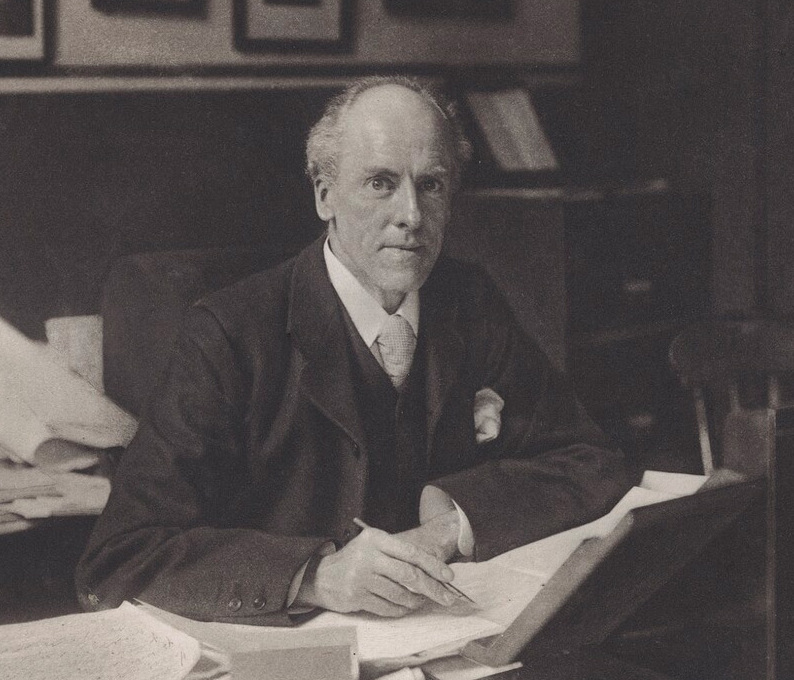
\includegraphics[width=7cm]{pearson}
	\end{figure}
	\begin{center}
		Professor Karl Pearson

		1857 - 1936
	\end{center}
\end{frame}

\begin{frame}
	\LARGE
	\vspace{2cm}
	\begin{center}
		\textcolor{SecondColor}{
			``Beware of attempts to interpret correlations between ratios
			whose numerators and denominators contain common parts''
		}
	\end{center}

	\vspace{3.55cm}
	\large
	\begin{flushright}
		\cite{Pearson1897}
	\end{flushright}
\end{frame}

\begin{frame}{Compositional Data}
	\LARGE
	Any measurement that can be described as parts or percentages of a whole

	\vspace{5mm}
	Often has units of \%, ppm or ppb
\end{frame}

\begin{frame}{Aitchison's Observation}
	\LARGE
	\vspace{1cm}
	Compositional data provide information only about the relative
	magnitudes of the parts, not their absolute values.

	\vspace{5mm}
	The information provided is essentially about \textit{ratios} 
	of the the components.

	\vspace{1.62cm}
	\large
	\begin{flushright}
		\cite{Aitchison2005}
	\end{flushright}
\end{frame}

\begin{frame}{Scale Invariance}
	\LARGE
	Compositional problems imply that the sizes of specimens are irrelevant.

	\begin{equation*}
		f(pw) = f(w) \quad \forall \,\, p > 0
	\end{equation*}

	\vspace{5mm}
	$f$ must be invariant under the group of scale transformations.
\end{frame}

\begin{frame}
	\LARGE
	\begin{center}
		\textit{
			Any meaningful (scale-invariant) function of a composition
			can be expressed in terms of ratios of the components of the
			composition.
		}
	\end{center}
\end{frame}

\begin{frame}{Subcompositional Coherence}
	\LARGE
	Subcompositions of a total composition must be consistent
	with other subcompositions of the same components.

	\vspace{5mm}
	Ratios between shared components stay the same.
\end{frame}

\begin{frame}{Aitchison's Observation}
	\LARGE
	\begin{center}
		\textit{
			Compositions contain information only about the relative
			magnitudes of the compositional components
		}
	\end{center}
\end{frame}

\begin{frame}[plain]
	\large
	\vspace{5mm}
	\begin{figure}
		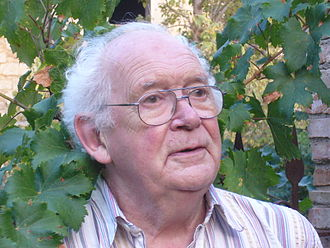
\includegraphics[width=8cm]{aitchison}
	\end{figure}
	\begin{center}
		John Aitchison

		1926 - 2016
	\end{center}
\end{frame}

\begin{frame}{Vector Space Structure}
	\LARGE
	Define the $D$ part simplex
	\Large
	\begin{equation*}
		\mathcal{S}^D = \left\{ \mathbf{x} = [x_1, x_2, \ldots , x_D];
		x_i > 0, i = 1, 2, \ldots , D; \sum^D_{i=1} x_i
		= \kappa \right\}
	\end{equation*}

	\LARGE
	\vspace{3mm}
	For $\kappa$ an arbitrary positive constant.
\end{frame}

\begin{frame}{Compositions}
	\LARGE
	Elements of $\mathcal{S}^D$ are called $D$-part compositions
\end{frame}

\begin{frame}{Vector Spaces}
	\LARGE
	Must haves to qualify as vector space
	\begin{enumerate}
		\item \textit{Non-empty} in field $F$
		\item \textit{binary operation} (often called vector addition)
		\item \textit{binary function} (often called scalar multiplication)
	\end{enumerate}
\end{frame}

\begin{frame}{Eight Axioms}
	\LARGE
	Every vector space $V$ over a field $F$ must satisfy
	the following eight axioms for $\mathbf{u}, \mathbf{v}, 
	\mathbf{w} \in V$ and $a, b \in F$
\end{frame}

\begin{frame}
	\LARGE
	\vspace{5mm}
	\begin{center}
		\renewcommand*{\arraystretch}{1.1}
		\begin{tabular}{|c|c|}
			\hline
			\textbf{Vector Addition} & \textbf{Scalar Multiplication} \\
			\hline
			\begin{tabular}{@{}c@{}}
				Associativity \\ $\mathbf{u} + (\mathbf{v} + \mathbf{w}) = (\mathbf{u} + \mathbf{v}) + \mathbf{w}$ 
			\end{tabular} & 
			\begin{tabular}{@{}c@{}}
				Compatibility \\ $a (b\mathbf{v}) = (ab) \mathbf{v}$
			\end{tabular} \\
			\hline
			\begin{tabular}{@{}c@{}}
				Commutativity \\ $\mathbf{u} + \mathbf{v} = \mathbf{v} + \mathbf{u}$
			\end{tabular} & 
			\begin{tabular}{@{}c@{}}
				Identity Element \\ $1\mathbf{v} = \mathbf{v}$
			\end{tabular} \\
			\hline
			\begin{tabular}{@{}c@{}}
				Identity Element \\ $\mathbf{v} + \mathbf{0} = \mathbf{v}$
			\end{tabular} & 
			\begin{tabular}{@{}c@{}}
				Distributivity (1) \\ $a(\mathbf{u} + \mathbf{v}) = a\mathbf{u} + a\mathbf{v}$
			\end{tabular} \\
			\hline
			\begin{tabular}{@{}c@{}}
				Inverse Element \\ $\mathbf{v} + (-\mathbf{v}) = 0$
			\end{tabular} & 
			\begin{tabular}{@{}c@{}}
				Distributivity (2) \\ $(a + b) \mathbf{v} = a\mathbf{v} + b\mathbf{v}$
			\end{tabular} \\
			\hline
		\end{tabular}
	\end{center}
\end{frame}

\begin{frame}{Vector Addition on $\mathcal{S}^D$}
	\LARGE
	On the simplex, vector addition is called
	\textcolor{ThirdColor}{perturbation}
	\begin{equation*}
		\mathbf{x} \oplus \mathbf{y} = \closure
		[x_1 y_1, x_2 y_2, \ldots , x_D y_D]
	\end{equation*}

	\vspace{4mm}
	$\closure(\cdot)$ denotes the \textcolor{ThirdColor}{closure}
	of a vector
\end{frame}

\begin{frame}{Closure}
	\LARGE
	The \textcolor{ThirdColor}{closure} operation divides
	all elements of a vector by the sum and then multiplies
	by $\kappa$
\end{frame}

\begin{frame}{Scalar Multiplication on $\mathcal{S}^D$}
	\LARGE
	On the simplex, scalar multiplication is called
	\textcolor{ThirdColor}{powering}
	\begin{equation*}
		\alpha \otimes \mathbf{x} = \closure[ x_1^\alpha,
		x_2^\alpha, \ldots , x_D^\alpha]
	\end{equation*}
\end{frame}

\begin{frame}
	\LARGE
	\vspace{1cm}
	For completeness sake, the identity element is
	\begin{equation*}
		\closure[1, 1, \ldots, 1]
	\end{equation*}

	\vspace{5mm}
	and the inverse of $\mathbf{y}$ is
	\begin{equation*}
		\mathbf{x} \ominus \mathbf{y} = \mathbf{x} \oplus
		((-1) \otimes \mathbf{y}) = \mathbf{x} \oplus
		\mathbf{y}^{-1}
	\end{equation*}
\end{frame}

\begin{frame}{Hilbert Space in $\mathcal{S}^D$}
	\LARGE
	The inner product on $\mathcal{S}^D$ is
	\begin{equation*}
		\langle \mathbf{x}, \mathbf{y} \rangle_a = 
		\frac{1}{D} \sum_{i < j} \log \frac{x_i}{x_j} 
		\log \frac{y_i}{y_j} = \sum^D_{i=1}
		\log \frac{x_i}{g(\mathbf{x})} \log \frac{y_i}
		{g(\mathbf{y})}
	\end{equation*}

	\vspace{5mm}
	Where $g(\mathbf{x}) = ( \prod_{i=1}^D x_i )^{1/D}$ is the 
	geometric mean
\end{frame}

\begin{frame}
	\LARGE
	Since any finite dimensional vector space with inner product
	is a Euclidean vector space and is complete, $\mathcal{S}^D$
	is a ($D-1$) dimensional Hilbert space. 
\end{frame}

\begin{frame}{Distance on $\mathcal{S}^D$}
	\LARGE
	\vspace{5mm}
	The inner product induces a norm and distance
	\begin{equation*}
		\| \mathbf{x} \|^2_a = \langle \mathbf{x}, \mathbf{x}
		\rangle_a
	\end{equation*}
	\begin{equation*}
		d_a(\mathbf{x}, \mathbf{y}) = \| \mathbf{x} \ominus
		\mathbf{y} \|_a
	\end{equation*}

	\vspace{5mm}
	Because the norm is invariant under permutation, so are
	the norm and distance operators
	\begin{gather*}
		d_a(\mathbf{s} \oplus \mathbf{x}, \mathbf{s} \oplus
		\mathbf{y}) = d_a(\mathbf{x}, \mathbf{y}) \\
		d_a(\alpha \otimes \mathbf{x}, \alpha \otimes
		\mathbf{y}) = |\alpha| d_a(\mathbf{x}, \mathbf{y})
	\end{gather*}
\end{frame}

\begin{frame}{Aitchison Geometry}
	\LARGE
	\vspace{1cm}
	$d_a$ is often called the \textcolor{ThirdColor}{Aitchison
	distance} in $\mathcal{S}^D$

	\vspace{5mm}
	Therefore the Hilbert geometry of $\mathcal{S}^D$ is called
	the \textcolor{ThirdColor}{Aitchison geometry}

	\vspace{3.18cm}
	\large
	\begin{flushright}
		\cite{Pawlowsky-Glahn2007}
	\end{flushright}
\end{frame}

\begin{frame}{Straight Lines in $\mathcal{S}^D$}
	\LARGE
	The \textcolor{SecondColor}{geodesic} from $\mathbf{x}_0$
	to $\mathbf{x}(t)$ is contained in
	\begin{equation*}
		\mathbf{x}(t) = \mathbf{x}_0 \oplus (t \otimes \mathbf{p})
		\quad \quad t \in \mathbb{R} \quad \mathbf{x}_0, \mathbf{p} \in
		\mathcal{S}^D
	\end{equation*}
\end{frame}

\begin{frame}{Orthogonality in $\mathcal{S}^D$}
	\LARGE
	For two orthogonal directions $\mathbf{p}_1, \mathbf{p}_2 \in
	\mathcal{S}^D$
	\begin{equation*}
		\langle \mathbf{p}_1, \mathbf{p}_2 \rangle_a = 0
	\end{equation*}

	\vspace{2mm}
	Two lines with the same direction $\mathbf{p}$ would be said
	to be parallel
\end{frame}

\begin{frame}
	\LARGE
	\begin{center}
		\textcolor{SecondColor}{
			\textbf{THOUGHT}
		}

		\vspace{5mm}
		Subcompositions of $\mathcal{S}^D$ should be ``orthogonal''
	\end{center}
\end{frame}

\begin{frame}{Linear Algebra}
	\LARGE
	Consider the linear combination in $\mathcal{S}^D$
	\begin{equation*}
		x = (u_1 \otimes \beta_1) \oplus \ldots \oplus 
		(u_C \otimes \beta_C)
	\end{equation*}

	\vspace{4mm}
	$\beta$'s are regarded as the composition's \textit{generators}
\end{frame}

\begin{frame}{Linear Algebra: $\range(B)$}
	\LARGE
	Consider orthonormal $B = \{ \beta_i \}_{i=1}^C$
	\begin{equation*}
		\range(B) = \{ x : x = (u_1 \otimes \beta_1) \oplus
		\ldots \oplus (u_C \otimes \beta_C), u_i \in \mathbb{R} \}
	\end{equation*}

	The generators in $B$ identify a range subspace of dimension
	$C$
\end{frame}

\begin{frame}{Linear Algebra: $\mnull(B)$}
	\LARGE
	\vspace{5mm}
	The generators also have an associated null space of
	dimension $D - C - 1$
	\begin{equation*}
		\mnull(B) = \{ x : \langle \beta_1, x \rangle = 0, \ldots ,
		\langle \beta_C, x \rangle = 0 \}
	\end{equation*}

	\vspace{5mm}
	Therefore
	\begin{align*}
		\range(B) &= \mnull(B^\perp) \\
		\mnull(B) &= \range(B^\perp)
	\end{align*}
\end{frame}

\begin{frame}{Additive Logratio Transform}
	\LARGE
	\begin{gather*}
		\alr(\mathbf{x}) = \left[ \log \frac{x_1}{x_D},
		\log \frac{x_2}{x_D}, \ldots , \log \frac{x_{D-1}}{x_D}
		\right] = \Theta \\[4mm]
		\alr^{-1}(\Theta) = \closure(\exp(\Theta_1), \ldots ,
		\exp(\Theta_{D-1}), 1) = \mathbf{x}
	\end{gather*}
\end{frame}

\begin{frame}{$\alr$}
	\LARGE
	Transforms perturbation and powering into standard operations
	in $\mathbb{R}$
	\begin{equation*}
		\alr[(\alpha \otimes \mathbf{x}) \oplus (\beta \otimes
		\mathbf{y})] = \alpha \alr \mathbf{x} + \beta \alr \mathbf{y}
	\end{equation*}
\end{frame}

\begin{frame}{$\alr$}
	\LARGE
	The transform is not permutation invariant, because the
	$D^\text{th}$ component normalizes all others

	\vspace{4mm}
	The transform is called \textcolor{ThirdColor}{asymmetric}

	\vspace{4mm}
	The $\alr$ is an isomorphism, but not an isometry 
\end{frame}

\begin{frame}{Centered Logratio Transform}
	\LARGE
	\begin{gather*}
		\clr(\mathbf{x}) = \left[ \log \frac{x_1}{g(\mathbf{x})},
		\log \frac{x_2}{g(\mathbf{x})}, \ldots , \frac{x_D}
		{g(\mathbf{x})} \right] = \xi \\[4mm]
		\clr^{-1}(\xi) = \closure[ \exp(\xi_1), \ldots ,
		\exp(\xi_D)] = \mathbf{x}
	\end{gather*}
\end{frame}

\begin{frame}{$\clr$}
	\LARGE
	Desirable properties
	\begin{align*}
		&\clr(\alpha \otimes \mathbf{x} \oplus \beta
		\otimes \mathbf{y}) = \alpha \clr \mathbf{x}
		+ \beta \clr \mathbf{y} \quad \quad \quad \quad \quad \\
		&\langle \mathbf{x}, \mathbf{y} \rangle_a =
		\langle \clr \mathbf{x}, \clr \mathbf{y} \rangle \\
		&\| \mathbf{x} \|_a = \| \clr \mathbf{x} \| \\
		&d_a( \mathbf{x}, \mathbf{y} ) = d(\clr \mathbf{x},
		\clr \mathbf{y} )
	\end{align*}
\end{frame}

\begin{frame}{$\clr$}
	\LARGE
	Symmetric in the components, unlike $\alr$

	\vspace{4mm}
	$\clr$ is an isometry, and therefore an isomorphism, but
	between $\mathcal{S}^D$ and a \textcolor{ThirdColor}{
		subspace} of $\mathbb{R}^D$. So the resulting basis
	is not orthonormal.
\end{frame}

\begin{frame}{$\clr$}
	\LARGE
	The transform imposes the constraint that the sum of
	$\xi$ is zero. Therefore, singular covariance matrices.

	\vspace{4mm}
	Worse, the $\clr$ coefficients are not subcompositionally
	coherent because the geometric mean will change.
\end{frame}

\begin{frame}
	\LARGE
	We desire a transformation to 
	\begin{enumerate}
		\item generate an orthonormal basis
		\item isometrically map from and to $\mathcal{S}^D$
	\end{enumerate}
\end{frame}

\begin{frame}[plain]
	\begin{figure}
		\begin{textblock*}{2.1cm}(0.1\paperwidth,0.2\paperheight)
			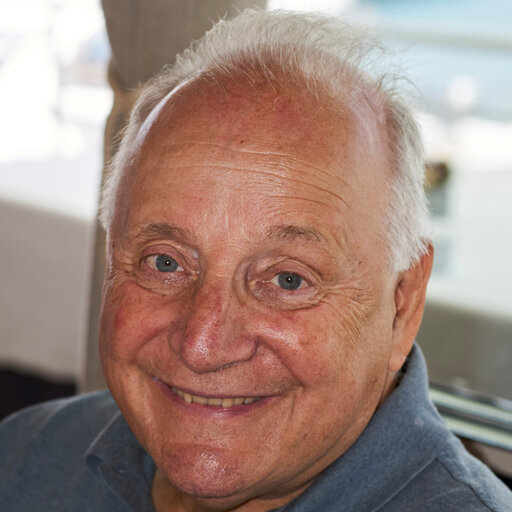
\includegraphics[width=2.4cm]{egozcue}
		\end{textblock*}
	\end{figure}
	\begin{figure}
		\begin{textblock*}{2.1cm}(0.31\paperwidth,0.3\paperheight)
			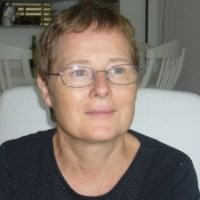
\includegraphics[width=2.4cm]{pawlowsky-glahn}
		\end{textblock*}
	\end{figure}
	\begin{figure}
		\begin{textblock*}{2.1cm}(0.525\paperwidth,0.2\paperheight)
			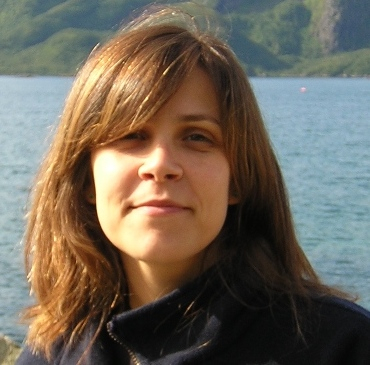
\includegraphics[width=2.4cm]{mateu-figueras}
		\end{textblock*}
	\end{figure}
	\begin{figure}
		\begin{textblock*}{2.1cm}(0.74\paperwidth,0.3\paperheight)
			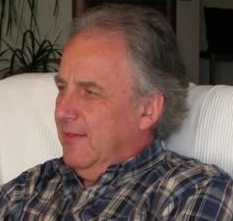
\includegraphics[width=2.4cm]{barcelo-vidal}
		\end{textblock*}
	\end{figure}
	\vspace{4cm}
	\begin{center}
		\Large
		Juan~Jos\'e~Egozcue, Vera~Pawlowsky-Glahn, 
		Gl\`oria~Mateu-Figueras, Carles~Barcel\'o-Vidal
	\end{center}
\end{frame}

\begin{frame}{Isometric Logratio Transform}
	\LARGE
	\vspace{5mm}
	Given composition $x \in \mathcal{S}^D$, the
	\textcolor{SecondColor}{isometric logratio transform}
	$\ilr : \mathcal{S}^D \rightarrow \mathbb{R}^{D-1}$ associated
	with an Aitchison-orthonormal basis $e_1, e_2, \ldots , e_{D-1}$
	\vspace{5mm}
	\begin{gather*}
		\mathbf{y} = \ilr(\mathbf{x}) = 
		[ \langle e_1, \mathbf{x} \rangle_a, \ldots ,
		\langle e_{D-1}, \mathbf{x} \rangle_a ] \\[4mm]
		\mathbf{x} = \ilr^{-1}(\mathbf{y}) = 
		\bigoplus_{i=1}^{D-1} ( \langle \mathbf{y}, e_i \rangle
		\otimes e_i )
	\end{gather*}

	\vspace{0.2mm}
	\large
	\begin{flushright}
		\cite{Egozcue2003}
	\end{flushright}
\end{frame}

\begin{frame}{$\ilr$}
	\LARGE
	\vspace{3mm}
	Desirable properties
	\begin{align*}
		&\ilr(\alpha \otimes \mathbf{x} \oplus \beta
		\otimes \mathbf{y}) = \alpha \ilr \mathbf{x}
		+ \beta \ilr \mathbf{y} \quad \quad \quad \quad \quad \\
		&\langle \mathbf{x}, \mathbf{y} \rangle_a =
		\langle \ilr \mathbf{x}, \ilr \mathbf{y} \rangle \\
		&\| \mathbf{x} \|_a = \| \ilr \mathbf{x} \| \\
		&d_a( \mathbf{x}, \mathbf{y} ) = d(\ilr \mathbf{x},
		\ilr \mathbf{y} )
	\end{align*}

	\vspace{5mm}
	\textcolor{SecondColor}{Just like $\clr$}
\end{frame}

\begin{frame}{$\ilr$ as modified $\clr$}
	\LARGE
	\begin{gather*}
		\mathbf{y} = \ilr(\mathbf{x}) = 
		\clr(\mathbf{x}) \cdot \Psi^T \\[2mm]
		\mathbf{x} = \ilr^{-1}(\mathbf{y}) =
		\clr^{-1}( \mathbf{y} \cdot \Psi )
	\end{gather*}

	\vspace{5mm}
	$\Psi \in \mathbb{R}^{(D-1) \times D}$ is called the 
	\textcolor{ThirdColor}{contrast matrix}
\end{frame}

\begin{frame}{The Contrast Matrix}
	\LARGE
	Contrast matrix $\Psi$ determines which on of
	an infinite number of orthonormal basis will span 
	$\mathcal{S}^D$

	\vspace{5mm}
	The rows of $\Psi$ are $\clr(e_i)$ and
	\begin{align*}
		\Psi \cdot \Psi^T &= \mathbf{I}_{D-1} \\
		\Psi^T \cdot \Psi &= \mathbf{I}_D - (1 / D) 
		\mathbf{1}^T_D \mathbf{1}_D
	\end{align*}
\end{frame}

\begin{frame}{The Contrast Matrix}
	\LARGE
	\vspace{1cm}
	\begin{center}
		So long as we obey these rules, \textit{we are free to
		determine the orthonormal basis $e_i$ and $\Psi$ ourselves}

		\vspace{5mm}
		\textcolor{ThirdColor}{
			In other words, inject prior information!
		}
	\end{center}

	\vspace{2.9cm}
	\large
	\begin{flushright}
		\cite{Chave2017}
	\end{flushright}
\end{frame}

\begin{frame}{Sequential Binary Partition}
	\LARGE
	$\Psi$ can be chosen by sequential binary partition.

	\vspace{5mm}
	This method enhances interpretability in the transform
	space, unlike principal component analysis.
\end{frame}

% Citations
\begin{frame}[allowframebreaks,plain]{References}
	\printbibliography
\end{frame}

\end{document}
